\chapter{Basic Concepts of Probability}

The theory of probability provides the mathematical tools necessary to study and analyze uncertain phenomena that occur in nature.
It establishes a formal framework to understand and predict the outcome of a random experiment.
It can be used to model complex systems and characterize stochastic processes.
This is instrumental in designing efficient solutions to many engineering problems.
Two components define a probabilistic model, a sample space and a probability law.


\section{Sample Spaces and Events}

In the context of probability, an \emph{experiment} is a random occurrence that produces one of several \emph{outcomes}.\index{Experiment}\index{Outcome}
The set of all possible outcomes is called the \emph{sample space} of the experiment, and it is denoted by $\Omega$.\index{Sample space}
An \emph{admissible} subset of the sample space is called an \emph{event}.\index{Event}

\begin{figure}[htb!]
\begin{center}
\begin{psfrags}
\psfrag{1}[c]{$1$}
\psfrag{2}[c]{$2$}
\psfrag{3}[c]{$3$}
\psfrag{4}[c]{$4$}
\psfrag{5}[c]{$5$}
\psfrag{6}[c]{$6$}
\psfrag{7}[c]{$7$}
\psfrag{E}[l]{event}
\psfrag{O}[r]{outcome}
\includegraphics[height=4.275cm]{Figures/2Chapter/samplespace}
\end{psfrags}
\caption{A sample space contains all the possible outcomes; an admissible subset of the sample space is called an event.}
\label{figure:SampleSpace}
\end{center}
\end{figure}

\begin{example}
The rolling of a die forms a common experiment.
A sample space $\Omega$ corresponding to this experiment is given by the six faces of a die.
The set of prime numbers less than or equal to six, namely $\{ 2, 3, 5 \}$, is one of many possible events.
The actual number observed after rolling the die is the outcome of the experiment.

\begin{figure}[htb!]
\begin{center}
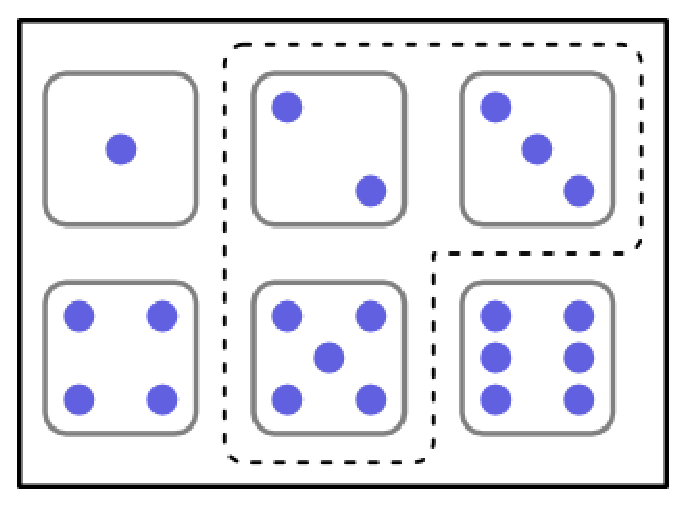
\includegraphics[height=3.38cm]{Figures/2Chapter/dices}
\caption{A possible sample space for the rolling of a die is $\Omega = \{ 1, 2, \ldots, 6 \}$, and the subset $\{2, 3, 5 \}$ forms a specific event.}
\end{center}
\end{figure}
\end{example}

There is essentially no restriction on what constitutes an experiment.
The flipping of a coin, the flipping of $n$ coins, and the tossing of an infinite sequence of coins are all random experiments.
Also, two similar experiments may have different sample spaces.
A sample space $\Omega$ for observing the number of heads in $n$ tosses of a coin is $\{ 0, 1, \ldots, n \}$; however, when describing the complete history of the $n$ coin tosses, the sample space becomes much larger with $2^n$ distinct sequences of heads and tails.
Ultimately, the choice of a particular sample space depends on the properties one wishes to analyze.
Yet some rules must be followed in selecting a sample space.
\begin{enumerate}
\item The elements of a sample space should be \emph{distinct} and \emph{mutually exclusive}.
This ensures that the outcome of an experiment is unique.\index{Distinct elements}\index{Mutually exclusive}
\item A sample space must be \emph{collectively exhaustive}.
That is, every possible outcome of the experiment must be accounted for in the sample space.\index{Collectively exhaustive}
\end{enumerate}
In general, a sample space should be precise enough to distinguish between all outcomes of interest, while avoiding frivolous details.

\begin{example}
Consider the space composed of the odd integers located between one and six, the even integers contained between one and six, and the prime numbers less than or equal to six.
This collection cannot be a sample space for the rolling of a die because its elements are not mutually exclusive.
In particular, the numbers three and five are both odd and prime, while the number two is prime and even.
This violates the uniqueness criterion.

\begin{figure}[htb!]
\begin{center}
\includegraphics[height=4.125cm]{Figures/2Chapter/nonadmissiblespace}
\caption{This collection of objects cannot be a sample space as the three proposed outcomes (even, odd and prime) are not mutually exclusive.}
\end{center}
\end{figure}

Alternatively, the elements of the space composed of the odd numbers between one and six, and the even numbers between one and six, are distinct and mutually exclusive;
an integer cannot be simultaneously odd and even.
Moreover, this space is collectively exhaustive because every integer is either odd or even.
This latter description forms a possible sample space for the rolling of a die.

\begin{figure}[htb!]
\begin{center}
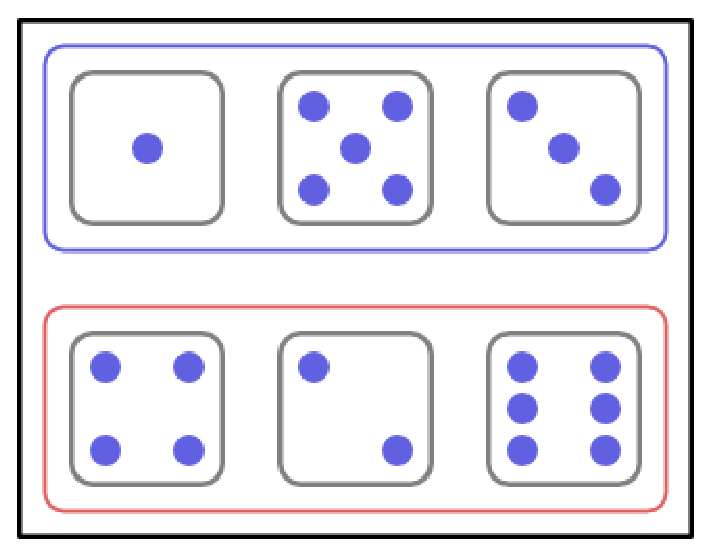
\includegraphics[height=3.75cm]{Figures/2Chapter/admissiblespace}
\end{center}
\caption{A candidate sample space for the rolling of a die is composed of two objects, the odd numbers and the even numbers between one and six.}
\end{figure}
\end{example}


\section{Probability Laws}
\label{section:ProbabilityLaws}

A \emph{probability law} specifies the likelihood of events related to an experiment.\index{Probability law}
Formally, a probability law assigns to every event $A$ a number $\Pr (A)$, called the \emph{probability of event $A$}, such that the following axioms are satisfied.
\begin{enumerate}
\item \textbf{(Nonnegativity)} $\Pr (A) \geq 0$, for every event $A$.
\item \textbf{(Normalization)} The probability of the sample space $\Omega$ is equal to one,
\begin{equation*}
\Pr (\Omega) = 1 .
\end{equation*}
\item \textbf{(Countable Additivity)} If $A$ and $B$ are disjoint events, $A \cap B = \emptyset$, then the probability of their union satisfies
\begin{equation*}
\Pr (A \cup B) = \Pr (A) + \Pr (B) .
\end{equation*}
More generally, if $A_1, A_2, \ldots$ is a sequence of disjoint events and $\bigcup_{k=1}^{\infty} A_k$ is itself an admissible event then
\begin{equation*}
\Pr \left( \bigcup_{k=1}^{\infty} A_k \right)
= \sum_{k = 1}^{\infty} \Pr (A_k) .
\end{equation*}
\end{enumerate}

A number of important properties can be deduced from the three axioms of probability.
We prove two such properties below.
The first statement describes the relation between inclusion and probabilities.
\begin{proposition}
If $A \subset B$, then $\Pr (A) \leq \Pr (B)$.
\end{proposition}
\begin{proof}
Since $A \subset B$, we have $B = A \cup (B - A)$.
Noting that $A$ and $B - A$ are disjoint sets, we get
\begin{equation*}
\Pr (B) = \Pr (A) + \Pr (B - A) \geq \Pr (A) ,
\end{equation*}
where the inequality follows from the nonnegativity of probability laws.
\end{proof}
\begin{figure}[htb!]
\begin{center}
\begin{psfrags}
\psfrag{A}[c]{$A$}
\psfrag{B}[l]{$B$}
\psfrag{D}[l]{$B - A$}
\includegraphics[height=3.03cm]{Figures/2Chapter/subset}
\end{psfrags}
\caption{If event $A$ is a subset of event $B$, then the probability of $A$ is less than or equal to the probability of $B$.}
\end{center}
\end{figure}

Our second result specifies the probability of the union of two events that are not necessarily mutually exclusive.
\begin{proposition} \label{proposition:ProbabilityUnion}
$\Pr (A \cup B) = \Pr (A) + \Pr (B) - \Pr (A \cap B)$.
\end{proposition}
\begin{proof}
Using the third axiom of probability on the disjoint sets $A$ and $(A \cup B) - A$, we can write
\begin{equation*}
\Pr (A \cup B)
= \Pr (A) + \Pr ((A \cup B) - A)
= \Pr (A) + \Pr (B - A) .
\end{equation*}
Similarly, applying the third axiom to $A \cap B$ and $B - (A \cap B)$, we obtain
\begin{equation*}
\Pr (B)
= \Pr (A \cap B) + \Pr (B - (A \cap B))
= \Pr (A \cap B) + \Pr (B - A) .
\end{equation*}
Combining these two equations yields the desired result.
\end{proof}
\begin{figure}[htb!]
\begin{center}
\begin{psfrags}
\psfrag{A}[r]{$A$}
\psfrag{B}[l]{$B$}
\psfrag{I}[c]{$A \cap B$}
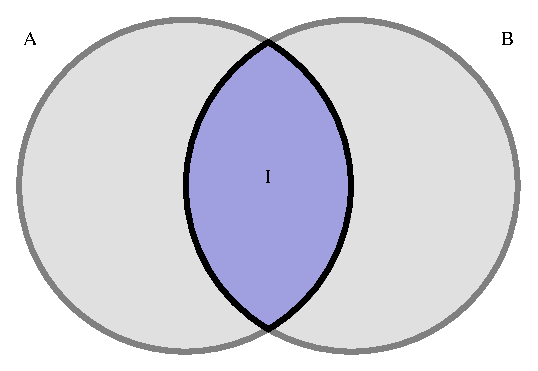
\includegraphics[height=3.03cm]{Figures/2Chapter/intersection}
\end{psfrags}
\caption{The probability of the union of $A$ and $B$ is equal to the probability of $A$ plus the probability of $B$ minus the probability of their intersection.}
\end{center}
\end{figure}

The statement of Proposition~\ref{proposition:ProbabilityUnion} can be extended to finite unions of events.
Specifically, we can write
\begin{equation*}
\Pr \left( \bigcup_{k=1}^{n} A_k \right)
= \sum_{k = 1}^{n} (-1)^{k-1} \sum_{\IndexSet \subset \{1, \ldots, n \}, |\IndexSet| =k } \Pr \left( \bigcap_{i \in \IndexSet} A_i \right)
\end{equation*}
where the rightmost sum runs over all subsets $\IndexSet$ of $\{ 1, \ldots, n \}$ that contain exactly $k$ elements.
This more encompassing result is known as the \emph{inclusion-exclusion principle}.\index{Inclusion-exclusion principle}

We can use Proposition~\ref{proposition:ProbabilityUnion} recursively to derive a bound on the probabilities of unions.
This theorem, which is sometimes called the \emph{Boole inequality}, asserts that the probability of at least one event occurring is no greater than the sum of the probabilities of the individual events.\index{Boole inequality}

\begin{theorem}[Union Bound]\index{Union bound}
Let $A_1, A_2, \ldots, A_n$ be a collection of events, then
\begin{equation} \label{equation:UnionBound}
\Pr \left( \bigcup_{k=1}^{n} A_k \right)
\leq \sum_{k = 1}^{n} \Pr (A_k) .
\end{equation}
\end{theorem}
\begin{proof}
We show this result using induction.
First, we note that the claim is trivially true for $n = 1$.
As an inductive hypothesis, assume that \eqref{equation:UnionBound} holds for some $n \geq 1$.
Then, we have
\begin{equation*}
\begin{split}
\Pr \left( \bigcup_{k=1}^{n+1} A_k \right)
&= \Pr \left( A_{n+1} \cup \left( \bigcup_{k=1}^{n} A_k \right) \right) \\
&= \Pr (A_{n+1}) + \Pr \left( \bigcup_{k=1}^{n} A_k \right)
- \Pr \left( A_{n+1} \cap \left( \bigcup_{k=1}^{n} A_k \right) \right) \\
&\leq \Pr (A_{n+1}) + \Pr \left( \bigcup_{k=1}^{n} A_k \right)
\leq \sum_{k = 1}^{n+1} \Pr (A_k) .
\end{split}
\end{equation*}
Therefore, by the principle of mathematical induction, \eqref{equation:UnionBound} is valid for all positive integers.
\end{proof}


\subsection{Finite Sample Spaces}
\label{section:FiniteSampleSpaces}

If a sample space $\Omega$ contains a finite number of elements, then a probability law on $\Omega$ is completely determined by the probabilities of its individual outcomes.
Denote a sample space containing $n$ elements by $\Omega = \{ s_1, s_2, \ldots, s_n \}$.
Any event in $\Omega$ is of the form $A = \{ s_i \in \Omega | i \in \IndexSet \}$, where $\IndexSet$ is a subset of the integers one through $n$.
The probability of event $A$ is therefore given by the third axiom of probability,
\begin{equation*}
\Pr (A)
= \Pr ( \{ s_i \in \Omega | i \in \IndexSet \} )
= \sum_{i \in \IndexSet} \Pr (s_i) .
\end{equation*}
We emphasize that, by definition, distinct outcomes are always disjoint events.

If in addition the elements of $\Omega$ are equally likely with
\begin{equation*}
\Pr (s_1) = \Pr (s_2) = \cdots = \Pr (s_n) = \frac{1}{n} ,
\end{equation*}
then the probability of an event $A$ becomes
\begin{equation} \label{equation:ProbEquiProbableOutcomes}
\Pr (A) = \frac{ |A| }{n}
\end{equation}
where $|A|$ denotes the number of elements in $A$.

\begin{example}
The rolling of a fair die is an experiment with a finite number of equally likely outcomes.
The probability of observing any of the faces labeled one through six is therefore equal to $1/6$.
The probability of any event can easily be computed by counting the number of distinct outcomes included in the event.
For instance, the probability of rolling a prime number is
\begin{equation*}
\Pr ( \{ 2, 3, 5 \} )
= \Pr (2) + \Pr(3) + \Pr(5) = \frac{3}{6} .
\end{equation*}
\end{example}


\subsection{Countably Infinite Models}

Consider a sample space that consists of a countably infinite number of elements, $\Omega = \{ s_1, s_2, \ldots \}$.
Again, a probability law on $\Omega$ is specified by the probabilities of individual outcomes.
An event in $\Omega$ can be written as $A = \{ s_j \in \Omega | j \in \JndexSet \}$, where $\JndexSet$ is a subset of the positive integers.
Using the third axiom of probability, $\Pr (A)$ can be written as
\begin{equation*}
\Pr (A)
= \Pr ( \{ s_j \in \Omega | j \in \JndexSet \} )
= \sum_{j \in \JndexSet} \Pr (s_j) .
\end{equation*}
The possibly infinite sum $\sum_{j \in \JndexSet} \Pr (s_j)$ always converges since the summands are nonnegative and the sum is bounded above by one; it is consequently well defined.

\begin{figure}[htb!]
\begin{center}
\begin{psfrags}
\psfrag{1}[c]{$1$}
\psfrag{2}[c]{$2$}
\psfrag{3}[c]{$3$}
\psfrag{4}[c]{$4$}
\psfrag{5}[c]{$5$}
\psfrag{6}[c]{$6$}
\psfrag{7}[c]{$7$}

\includegraphics[height=0.765cm]{Figures/2Chapter/countablespace}
\end{psfrags}
\caption{A countable set is a collection of elements with the same cardinality as some subset of the natural numbers.}
\end{center}
\end{figure}

\begin{example} \label{example:CoinTossSequence}
Suppose that a fair coin is tossed repetitively until heads is observed.
The number of coin tosses is recorded as the outcome of this experiment.
A natural sample space for this experiment is $\Omega = \{ 1, 2, \ldots \}$, a countably infinite set.

The probability of observing heads on the first trial is $1/2$, and the probability of observing heads for the first time on trial $k$ is $2^{-k}$.
The probability of the entire sample space is therefore equal to
\begin{equation*}
\Pr ( \Omega ) = \sum_{k=1}^{\infty} \Pr (k)
= \sum_{k=1}^{\infty} \frac{1}{2^k} = 1 ,
\end{equation*}
as expected.
Similarly, the probability of the number of coin tosses being even can be computed as
\begin{equation*}
\Pr ( \{ 2, 4, 6, \ldots \} )
= \sum_{k=1}^{\infty} \Pr (2k)
= \sum_{k = 1}^{\infty} \frac{1}{2^{2k}}
= \frac{1}{4} \frac{1}{ \left( 1 - \frac{1}{4} \right) }
= \frac{1}{3} .
\end{equation*}
\end{example}


\subsection{Uncountably Infinite Models}

Probabilistic models with uncountably infinite sample spaces differ from the finite and countable cases in that a probability law may not necessarily be specified by the probabilities of single-element outcomes.
This difficulty arises from the large number of elements contained in the sample space when the latter is uncountable.
Many subsets of $\Omega$ do not have a finite or countable representation, and as such the third axiom of probability cannot be applied to relate the probabilities of these events to the probabilities of individual outcomes.
Despite these apparent difficulties, probabilistic models with uncountably infinite sample spaces are quite useful in practice.
To develop an understanding of uncountable probabilistic models, we consider the unit interval $[0, 1]$.

\begin{figure}[htb!]
\begin{center}
\begin{psfrags}
\psfrag{0}[c]{$0$}
\psfrag{1}[c]{$1$}
\includegraphics[height=1.17cm]{Figures/2Chapter/uncountablespace}
\end{psfrags}
\caption{The unit interval $[0,1]$, composed of all real numbers between zero and one, is an example of an uncountable set.}
\end{center}
\end{figure}

Suppose that an element is chosen at random from this interval, with uniform weighting.
By the first axiom of probability, the probability that this element belongs to the interval $[0,1]$ is given by $\Pr \left( [0,1] \right) = 1$.
Furthermore, if two intervals have the same length, the probabilities of the outcome falling in either interval should be identical.
For instance, it is natural to anticipate that $\Pr \left( \left( 0, 0.25 \right) \right) = \Pr \left( \left( 0.75, 1 \right) \right)$.

\begin{figure}[htb!]
\begin{center}
\begin{psfrags}
\psfrag{0}[l]{$0$}
\psfrag{0.25}[r]{$0.25$}
\psfrag{0.75}[l]{$0.75$}
\psfrag{1}[r]{$1$}
\includegraphics[height=1.185cm]{Figures/2Chapter/intervals}
\end{psfrags}
\caption{If the outcome of an experiment is uniformly distributed over $[0,1]$, then two subintervals of equal lengths should have the same probabilities.}
\end{center}
\end{figure}

In an extension of the previous observation, we take the probability of an open interval $(a, b)$ where $0 \leq a < b \leq 1$ to equal
\begin{equation} \label{equation:DefinitionProbabilityLaw1}
\Pr ( (a,b) ) = b - a .
\end{equation}
Using the third axiom of probability, it is then possible to find the probability of a finite or countable union of disjoint open intervals.

\begin{figure}[htb!]
\begin{center}
\begin{psfrags}
\psfrag{0}[l]{$0$}
\psfrag{1}[r]{$1$}
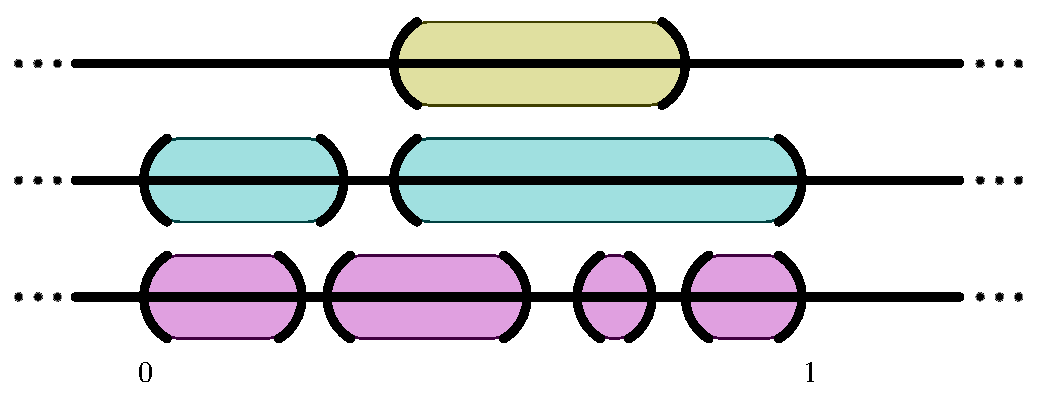
\includegraphics[height=3.28cm]{Figures/2Chapter/lineintervals}
\end{psfrags}
\caption{The probabilities of events that are formed through the union of disjoint intervals can be computed in a straightforward manner.}
\end{center}
\end{figure}

Specifically, for constants $0 \leq a_1 < b_1 < a_2 < b_2 < \cdots \leq 1$, we get
\begin{equation*}
\Pr \left( \bigcup_{k=1}^{\infty} (a_k,b_k) \right)
= \sum_{k=1}^{\infty} \left( b_k - a_k \right) .
\end{equation*}
The probabilities of more complex events can be obtained by applying additional elementary set operations.
However, it suffices to say for now that specifying the probability of the outcome falling in $(a,b)$ for every possible open interval is enough to define a probability law on $\Omega$.
In the example at hand, \eqref{equation:DefinitionProbabilityLaw1} completely determines the probability law on $[0,1]$.

Note that we can give an alternative means of computing the probability of an interval.
Again, consider the open interval $(a, b)$ where $0 \leq a < b \leq 1$.
The probability of the outcome falling in this  interval is equal to
\begin{equation*}
\Pr ( (a, b) ) = b - a = \int_a^b dx = \int_{(a,b)} dx .
\end{equation*}
Moreover, for $0 \leq a_1 < b_1 < a_2 < b_2 < \cdots \leq 1$, we can write
\begin{equation*}
\Pr \left( \bigcup_{k=1}^{\infty} (a_k,b_k) \right)
= \sum_{k=1}^{\infty} \left( b_k - a_k \right)
= \int_{\bigcup_{k=1}^{\infty} (a_k,b_k)} dx .
\end{equation*}
For this carefully crafted example, it appears that the probability of an admissible event $A$ is given by the integral
\begin{equation*}
\Pr (A) = \int_{A} dx .
\end{equation*}
This is indeed accurate for the current scenario.
In fact, the class of admissible events for this experiment is simply the collection of all sets for which the integral $\int_A dx$ can be computed.
In other words, if a number is chosen at random from $[0,1]$, then the probability of this number falling in measurable set $A \subset [0,1]$ is
\begin{equation*}
\Pr (A) = \int_{A} dx .
\end{equation*}
This method of computing probabilities can be extended to more complicated problems.
In these notes, we will see many probabilistic models with uncountably infinite sample spaces.
The mathematical tools required to handle such models will be treated alongside.

\begin{example}
Suppose that a participant at a game-show is required to spin the wheel of serendipity, a perfect circle with unit radius.
When subjected to a vigorous spin, the wheel is equally likely to stop anywhere along its perimeter.
A sampling space for this experiment is the collection of all angles from $0$ to $2 \pi$, an uncountable set.
The probability of $\Omega$ is invariably equal to one, $\Pr ([0, 2 \pi)) = 1$.

\begin{figure}[tbh!]
\begin{center}
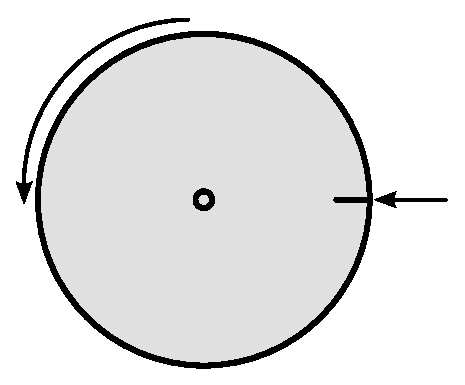
\includegraphics[height=3.15cm]{Figures/2Chapter/wheel}
\caption{The wheel of serendipity forms an example of a random experiment for which the sample space is uncountable.}
\end{center}
\end{figure}

The probability that the wheel stops in the first quadrant is given by
\begin{equation*}
\Pr \left( \left[ 0, \frac{\pi}{2} \right) \right)
= \int_{0}^{\frac{\pi}{2}} \frac{1}{2 \pi} d\theta
= \frac{1}{4}.
\end{equation*}
More generally, the probability that the wheel stops in an interval $(a, b)$ where $0 \leq a \leq b < 2 \pi$ can be written as
\begin{equation*}
\Pr ((a,b)) = \frac{b - a}{2 \pi}.
\end{equation*}
If $B \subset [0, 2 \pi)$ is a set representing all winning outcomes, then the probability of success at the wheel becomes
\begin{equation*}
\Pr(B) = \int_B \frac{1}{2 \pi} d\theta .
\end{equation*}
\end{example}


\subsection{Probability and Measure Theory*}

A thorough treatment of probability involves advanced mathematical concepts, especially when it comes to infinite sample spaces.
The basis of our intuition for the infinite is the set of \emph{natural numbers},\index{Natural numbers}
\begin{equation*}
\NaturalNumbers = \{ 1, 2, \ldots \}.
\end{equation*}
Two sets are said to have the same \emph{cardinality} if their elements can be put in one-to-one correspondence.\index{Cardinality}
A set with the same cardinality as a subset of the natural numbers is said to be \emph{countable}.\index{Countable}
That is, the elements of a countable set can always be listed in sequence, $s_1, s_2, \ldots$; although the order may have nothing to do with any relation between the elements.
The integers and the rational numbers are examples of countably infinite sets.
It may be surprising at first to learn that there exist uncountable sets.
To escape beyond the countable, one needs set theoretic tools such as \emph{power sets}.\index{Power set}
The set of real numbers is uncountably infinite; it cannot be put in one-to-one correspondence with the natural numbers.
A typical progression in analysis consists of using the finite to gain intuition about the countably infinite, and then to employ the countably infinite to get at the uncountable.

It is tempting to try to assign probabilities to every subset of a sample space $\Omega$.
However, for uncountably infinite sample spaces, this leads to serious difficulties that cannot be resolved.
In general, it is necessary to work with special subclasses of the class of all subsets of a sample space $\Omega$.
The collections of the appropriate kinds are called fields and $\sigma$-fields, and they are studied in \emph{measure theory}.\index{Measure theory}
This leads to measure-theoretic probability, and to its unified treatment of the discrete and the continuous.

Fortunately, it is possible to develop a working understanding of probability without worrying excessively about these issues.
At some point in your academic career, you may wish to study analysis and measure theory more carefully and in greater details.
However, it is not our current purpose to initiate the rigorous treatment of these topics.


\section*{Further Reading}

\begin{small}
\begin{enumerate}
\item Ross, S., \emph{A First Course in Probability}, 7th edition, Pearson Prentice Hall, 2006: Chapter~2.
\item Bertsekas, D. P., and Tsitsiklis, J. N., \emph{Introduction to Probability}, Athena Scientific, 2002: Section~1.2.
\item Miller, S. L., and Childers, D. G., \emph{Probability and Random Processes with Applications to Signal Processing and Communications}, 2004: Sections~2.1--2.3.
\item Gubner, J. A., \emph{Probability and Random Processes for Electrical and Computer Engineers}, Cambridge, 2006: Sections~1.1,1.3--1.4.
\end{enumerate}
\end{small}

